\chapter{Results and Discussion}
\label{ch:results}

This chapter reports the final held-out results of the three protocols (E1--E3, Table~\ref{tab:protocols}), compares the approach with existing methods, presents ablations and supporting analyses, and discusses what the evidence does and does not show. Unless stated otherwise, values are means over the six evaluation episodes; reward is per 500-step episode. Complete tables, including action counts, are given in Appendix~\ref{app:tables}.

\section{Overall Experimental Results}
\label{sec:overall}

\subsection{Training behaviour}

Figure~\ref{fig:training} shows the reward of every 1,000-step training episode for the selected synthetic models. The curves do not rise smoothly. Each training episode replays a different chronological window of the training trace, and the windows differ greatly in difficulty: a window that falls in a sustained peak cannot score as well as one in a quiet period, whatever the policy does. Training reward therefore mostly reflects the traffic window. It is not used here as evidence of learning; that evidence comes from comparing policies on identical held-out windows. The curves confirm that training was numerically stable, with no divergence or collapse, on every topology including the 197-switch Cogentco network.

\begin{figure}[htbp]
  \centering
  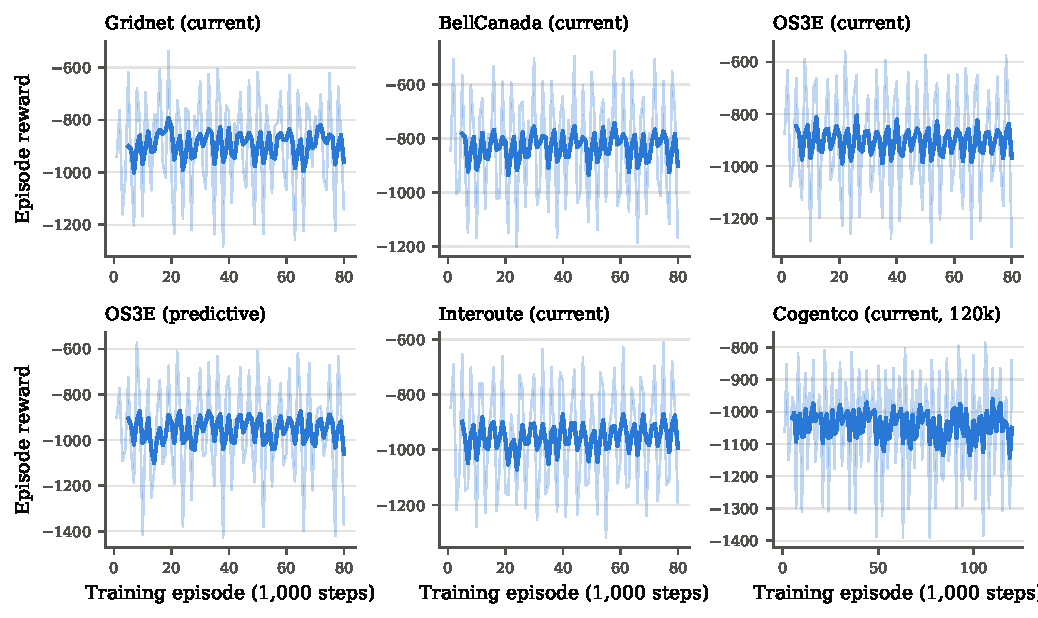
\includegraphics[width=\textwidth]{training_curves}
  \caption{Training-episode reward (light) and five-episode moving average (dark) for the selected synthetic models. Variation is dominated by the traffic window replayed in each episode.}
  \label{fig:training}
\end{figure}

\subsection{GRU forecasting quality}
\label{sec:res-gru}

Table~\ref{tab:gru} and Figure~\ref{fig:gru} compare the GRU forecasters with the persistence baseline on validation data. At horizon 5 the GRU reduced MAE by 15.6\% on Gridnet, 7.8\% on BellCanada and 8.5\% on OS3E, but was \emph{worse} than persistence on the two largest topologies (Interoute $-5.6$\%, Cogentco $-12.2$\%). Their traces are smoother, which makes persistence a strong forecaster, and one 64-unit GRU must model 110 and 197 correlated series. Predictive RDQN was therefore trained only for Gridnet, BellCanada and OS3E. Shortening the horizon to 3 improved Gridnet clearly but gave BellCanada almost no advantage over persistence. On the Abilene-derived trace the GRU had a slightly higher MAE than persistence but a lower RMSE and a higher overload F1 in all three seeds. In other words, it makes fewer large errors and detects more overload events, which is the property that matters for proactive decisions.

\begin{table}[htbp]
\centering
\caption{GRU forecaster versus persistence on validation data (history 12). Overload F1 is for predicting a switch load above 0.70. Bold marks the better of the pair.}
\label{tab:gru}
\small
\begin{tabular}{@{}llcccccc@{}}
\toprule
& & \multicolumn{2}{c}{\textbf{MAE}} & \multicolumn{2}{c}{\textbf{RMSE}} & \multicolumn{2}{c}{\textbf{Overload F1}}\\
\cmidrule(lr){3-4}\cmidrule(lr){5-6}\cmidrule(lr){7-8}
\textbf{Data} & \textbf{$h$} & GRU & Persist. & GRU & Persist. & GRU & Persist.\\
\midrule
Gridnet (syn.)    & 5 & \textbf{0.0345} & 0.0409 & \textbf{0.0487} & 0.0579 & \textbf{0.939} & 0.923\\
BellCanada (syn.) & 5 & \textbf{0.0360} & 0.0390 & \textbf{0.0504} & 0.0570 & \textbf{0.966} & 0.961\\
OS3E (syn.)       & 5 & \textbf{0.0356} & 0.0389 & \textbf{0.0537} & 0.0573 & \textbf{0.968} & 0.966\\
Interoute (syn.)  & 5 & 0.0370 & \textbf{0.0351} & 0.0561 & \textbf{0.0526} & 0.973 & \textbf{0.974}\\
Cogentco (syn.)   & 5 & 0.0361 & \textbf{0.0322} & 0.0549 & \textbf{0.0501} & 0.979 & \textbf{0.981}\\
\midrule
Gridnet (syn.)    & 3 & \textbf{0.0254} & 0.0299 & \textbf{0.0346} & 0.0411 & \textbf{0.953} & 0.944\\
BellCanada (syn.) & 3 & \textbf{0.0277} & 0.0278 & \textbf{0.0390} & 0.0397 & \textbf{0.974} & 0.972\\
\midrule
OS3E Abilene, seed 42 & 5 & 0.0294 & \textbf{0.0275} & \textbf{0.0416} & 0.0438 & \textbf{0.777} & 0.764\\
OS3E Abilene, seed 43 & 5 & 0.0294 & \textbf{0.0275} & \textbf{0.0424} & 0.0438 & \textbf{0.768} & 0.764\\
OS3E Abilene, seed 44 & 5 & 0.0296 & \textbf{0.0275} & \textbf{0.0424} & 0.0438 & \textbf{0.779} & 0.764\\
\bottomrule
\end{tabular}
\end{table}

\begin{figure}[htbp]
  \centering
  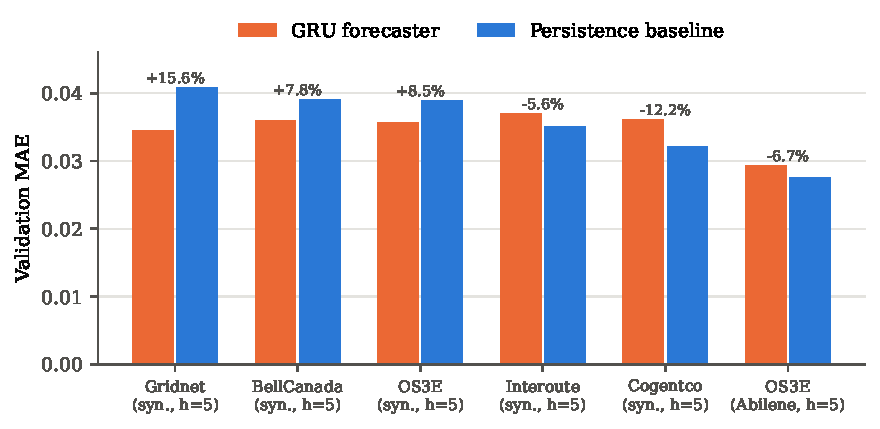
\includegraphics[width=0.92\textwidth]{gru_vs_persistence}
  \caption{Validation MAE of the GRU and the persistence forecast (horizon 5). Labels give the GRU's relative MAE improvement; negative values mean persistence is better.}
  \label{fig:gru}
\end{figure}

\subsection{E1: Synthetic held-out results across five topologies}
\label{sec:res-syn}

Table~\ref{tab:syn-main} reports the final test results for the selected learned policy of each topology against the three baselines evaluated under the same conditions. Figures~\ref{fig:syn-reward} and~\ref{fig:syn-metrics} show the same comparison graphically. The selected policy is current-state RDQN for four topologies and predictive GRU-RDQN for OS3E, following validation (Section~\ref{sec:ablation-mode}).

\begin{table}[htbp]
\centering
\caption{E1 final test on held-out synthetic traffic: selected learned policy versus baselines (six episodes $\times$ 500 steps, evaluation seed 2042). Best value per topology and metric in bold.}
\label{tab:syn-main}
\small
\fitwidth{\begin{tabular}{@{}llrrrrr@{}}
\toprule
\textbf{Topology} & \textbf{Policy} & \textbf{Reward}$\uparrow$ & \textbf{Avg lat.}$\downarrow$ & \textbf{Worst lat.}$\downarrow$ & \textbf{Energy}$\downarrow$ & \textbf{Load idx}$\downarrow$\\
 & & & (ms) & (ms) & (W) & \\
\midrule
\multirow{4}{*}{Gridnet} & Current RDQN & \textbf{$-$446.33} & 8.81 & 20.78 & 411.67 & 0.919\\
 & Threshold & $-$474.97 & 7.98 & 21.37 & 429.73 & 0.906\\
 & Random-valid & $-$464.30 & 8.23 & 21.09 & 423.13 & 0.922\\
 & No-op & $-$505.82 & \textbf{3.68} & \textbf{12.85} & \textbf{370.00} & \textbf{0.816}\\
\midrule
\multirow{4}{*}{BellCanada} & Current RDQN & \textbf{$-$384.27} & 11.51 & 34.86 & 398.11 & \textbf{6.162}\\
 & Threshold & $-$408.54 & 11.15 & 36.27 & 446.56 & 6.337\\
 & Random-valid & $-$424.66 & 11.63 & 33.16 & 447.85 & 6.216\\
 & No-op & $-$529.37 & \textbf{10.70} & \textbf{25.28} & \textbf{370.00} & 14.236\\
\midrule
\multirow{4}{*}{OS3E} & Predictive GRU-RDQN & \textbf{$-$452.94} & 4.54 & 15.89 & 380.89 & 4.223\\
 & Threshold (pred.) & $-$508.53 & 4.15 & 15.76 & 445.60 & \textbf{3.637}\\
 & Random-valid (pred.) & $-$515.07 & 4.54 & 15.76 & 447.22 & 4.403\\
 & No-op & $-$507.38 & \textbf{2.60} & \textbf{11.51} & \textbf{370.00} & 4.190\\
\midrule
\multirow{4}{*}{Interoute} & Current RDQN & \textbf{$-$477.57} & 6.01 & 17.38 & 383.38 & 19.353\\
 & Threshold & $-$529.96 & 5.79 & 17.38 & 461.02 & 18.709\\
 & Random-valid & $-$528.67 & 5.25 & 16.33 & 461.20 & 18.389\\
 & No-op & $-$499.02 & \textbf{4.39} & \textbf{14.57} & \textbf{370.00} & \textbf{18.117}\\
\midrule
\multirow{4}{*}{Cogentco} & Current RDQN (120k) & \textbf{$-$447.52} & 15.18 & 51.05 & 373.54 & 37.957\\
 & Threshold & $-$514.59 & 16.18 & 51.67 & 464.35 & 39.063\\
 & Random-valid & $-$522.46 & 15.96 & 57.01 & 463.33 & 37.305\\
 & No-op & $-$472.06 & \textbf{7.59} & \textbf{29.79} & \textbf{370.00} & \textbf{34.922}\\
\bottomrule
\end{tabular}}
\end{table}

\begin{figure}[htbp]
  \centering
  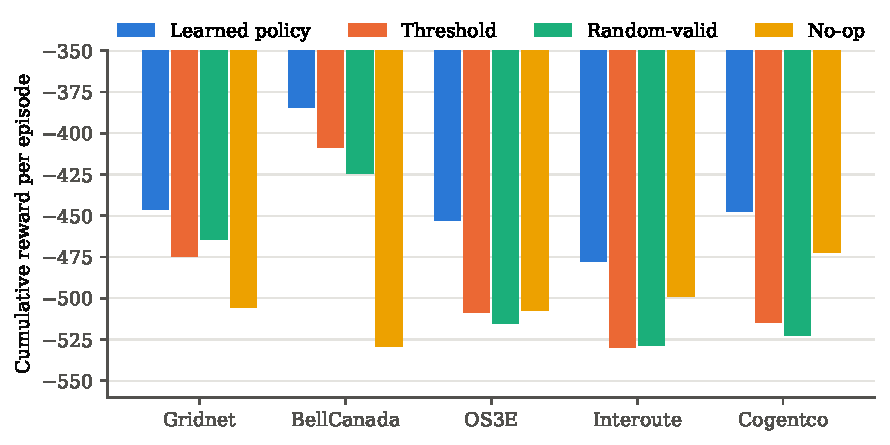
\includegraphics[width=\textwidth]{syn_reward}
  \caption{E1 final-test cumulative reward per episode (higher is better). The learned policy is current RDQN except for OS3E (predictive GRU-RDQN).}
  \label{fig:syn-reward}
\end{figure}

\begin{figure}[htbp]
  \centering
  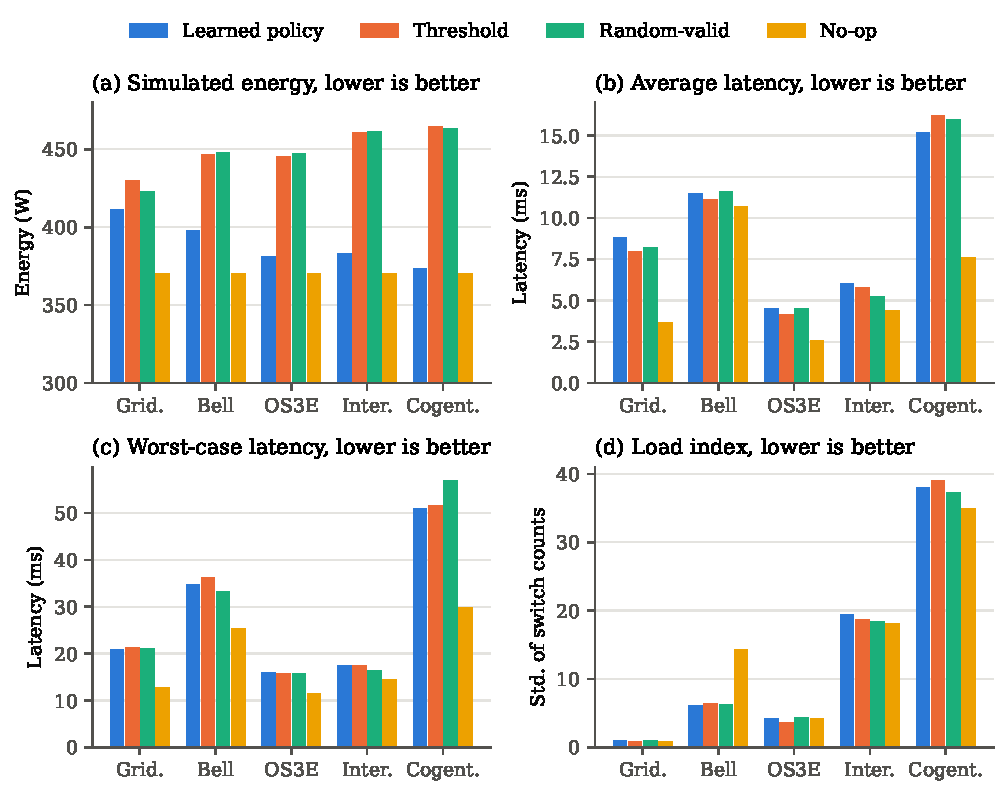
\includegraphics[width=\textwidth]{syn_metrics}
  \caption{E1 final-test operating metrics for the same policies as Figure~\ref{fig:syn-reward}.}
  \label{fig:syn-metrics}
\end{figure}

\paragraph{Principal finding.} The learned policy obtained the \textbf{highest reward on all five topologies}, ahead of all three baselines. Table~\ref{tab:syn-delta} expresses the result relative to the threshold policy, the strongest practical baseline. The learned policy consistently used less energy, from 18\,W (4.2\%) on Gridnet up to 91\,W (19.6\%) on Cogentco, and the saving grows with topology size. It achieved this mainly by keeping fewer controllers active: on Interoute and Cogentco its mean energy (383 and 374\,W) is close to the 370\,W of the initial three-controller state, whereas the threshold policy averaged more than 460\,W because it evokes whenever overload appears.

\begin{table}[htbp]
\centering
\caption{E1: change of the learned policy relative to the threshold baseline (learned minus threshold). Positive reward and negative energy/latency are improvements.}
\label{tab:syn-delta}
\small
\fitwidth{\begin{tabular}{@{}lrrrrr@{}}
\toprule
\textbf{Topology} & \textbf{$\Delta$Reward} & \textbf{$\Delta$Energy (W)} & \textbf{$\Delta$Avg lat. (ms)} & \textbf{$\Delta$Worst lat. (ms)} & \textbf{$\Delta$Load idx}\\
\midrule
Gridnet          & $+28.64$ & $-18.06$ ($-4.2$\%)  & $+0.83$ & $-0.59$ & $+0.013$\\
BellCanada       & $+24.27$ & $-48.45$ ($-10.8$\%) & $+0.36$ & $-1.41$ & $-0.175$\\
OS3E (predictive)& $+55.59$ & $-64.71$ ($-14.5$\%) & $+0.39$ & $+0.13$ & $+0.586$\\
Interoute        & $+52.40$ & $-77.64$ ($-16.8$\%) & $+0.22$ & $\phantom{+}0.00$ & $+0.644$\\
Cogentco         & $+67.07$ & $-90.81$ ($-19.6$\%) & $-1.00$ & $-0.61$ & $-1.106$\\
\bottomrule
\end{tabular}}
\end{table}

\paragraph{Trade-offs.} The learned policy does not win on every metric. Its average latency was 0.2--0.8\,ms higher than the threshold policy's on four topologies; Cogentco is the exception, with 1.0\,ms lower. Its worst-case latency was lower or equal on four topologies. Its count-based load index was mixed. These trade-offs are intended by the design: the reward weights energy and traffic balance alongside latency, and parking a controller necessarily moves its switches to more distant controllers.

\paragraph{The no-op reference.} No-op has the lowest latency and energy in every topology, because it keeps the initial nearest-controller assignment and never evokes extra controllers. It never responds to overload, which is present in 55--69\% of steps on this traffic, and never parks controllers during quiet periods, so its low latency and energy are not good controller management. Its reward is the worst of all policies on Gridnet and BellCanada. On OS3E, Interoute and Cogentco, however, no-op ranks \emph{second}, ahead of both active baselines. On those topologies, reacting to every overload by evoking costs more energy than it recovers, and the learned policy's restraint (few evokes, near-baseline energy) is what pays off. The no-op results show why individual metrics must be read together with the reward, and why simple reactivity is not automatically better than inaction.

\paragraph{Uncertainty.} The standard deviation of episode reward \emph{within} each evaluation is large (about 145--225 for the learned policies), because the six windows differ in traffic intensity. All policies see the same six windows, so the comparison is paired. Only per-window aggregates were stored, however, so a formal paired test is not possible from the saved results, and the synthetic results come from a single training seed. The margins over the threshold policy (24--67 reward points) are consistent in direction across five independent topologies, which supports the finding, but they are not a statistical significance claim.

\subsection{E2: Zero-shot transfer to Abilene-derived traffic}
\label{sec:res-zeroshot}

E2 tests whether the synthetic-trained OS3E policies still behave sensibly on real traffic dynamics they have never seen. Table~\ref{tab:zeroshot} and Figure~\ref{fig:zeroshot} give the results. In both modes the learned policy had the best reward and the lowest energy of all active policies. Predictive GRU-RDQN was marginally better than current RDQN on reward ($-74.62$ versus $-76.56$), energy ($-3.8$\,W), worst-case latency ($-0.63$\,ms) and load index (0.986 versus 1.548). The differences are small. Overload occurs in less than 1\% of steps on this trace, so the policies mainly had to decide when to park. The GRU's forecast error rose from 0.037 on synthetic OS3E to 0.176 here, a clear sign of distribution shift. E2 therefore shows that the policies \emph{transfer without failure}: they produce zero failed actions and still beat the baselines. It does not show that prediction generalises.

\begin{table}[htbp]
\centering
\caption{E2 zero-shot results on the Abilene-derived OS3E test trace (models trained on synthetic OS3E only).}
\label{tab:zeroshot}
\small
\fitwidth{\begin{tabular}{@{}llrrrrrr@{}}
\toprule
\textbf{Mode} & \textbf{Policy} & \textbf{Reward} & \textbf{Avg lat.} & \textbf{Worst lat.} & \textbf{Energy} & \textbf{Load idx} & \textbf{Under\%}\\
\midrule
\multirow{4}{*}{Current} & RDQN & \textbf{$-$76.56} & 6.45 & 18.14 & \textbf{218.65} & \textbf{1.548} & \textbf{9.8}\\
 & Threshold & $-$82.27 & 6.41 & 18.14 & 231.79 & 1.757 & 10.4\\
 & Random-valid & $-$82.44 & 6.22 & 17.51 & 229.21 & 2.238 & 10.3\\
 & No-op & $-$233.34 & 2.60 & 11.51 & 370.00 & 4.190 & 28.2\\
\midrule
\multirow{4}{*}{Predictive} & GRU-RDQN & \textbf{$-$74.62} & 6.39 & 17.51 & \textbf{214.81} & \textbf{0.986} & \textbf{10.1}\\
 & Threshold & $-$83.44 & 6.38 & 18.14 & 233.32 & 1.619 & 10.5\\
 & Random-valid & $-$90.73 & 6.45 & 18.14 & 235.06 & 2.477 & 11.3\\
 & No-op & $-$233.34 & 2.60 & 11.51 & 370.00 & 4.190 & 28.2\\
\bottomrule
\end{tabular}}
\par\smallskip\footnotesize Forecast MAE in predictive mode: 0.1764. Overload occurred in at most 0.6\% of steps for any policy.
\end{table}

\begin{figure}[htbp]
  \centering
  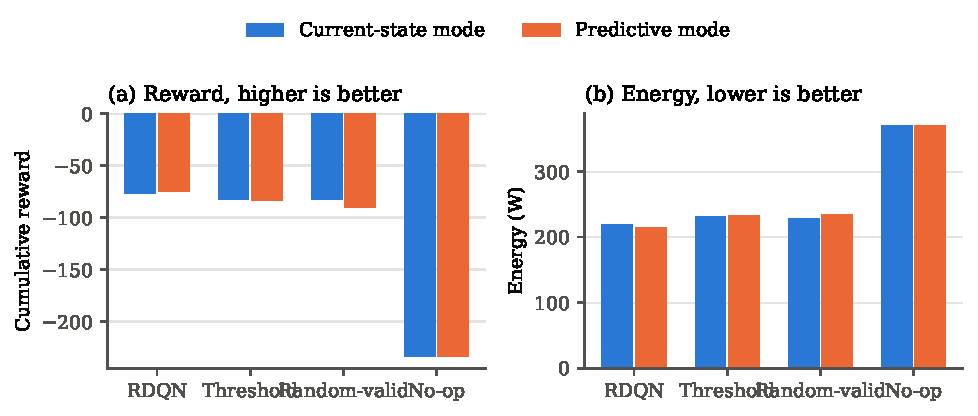
\includegraphics[width=0.95\textwidth]{zero_shot}
  \caption{E2 zero-shot reward and energy on the Abilene-derived OS3E test trace, by policy and observation mode.}
  \label{fig:zeroshot}
\end{figure}

\subsection{E3: Real-data-trained OS3E with three training seeds}
\label{sec:res-real}

In E3 the GRU, current RDQN and predictive GRU-RDQN were trained on Abilene-derived data and tested on the untouched final weeks \texttt{X21}--\texttt{X24}. The procedure was repeated for seeds 42, 43 and 44. Table~\ref{tab:real-agg} reports mean $\pm$ sample standard deviation, Table~\ref{tab:real-seed} reports the per-seed rewards, and Figure~\ref{fig:real} shows both.

\begin{table}[htbp]
\centering
\caption{E3 final test, mean $\pm$ sample s.d. across training seeds 42, 43 and 44. Both models had zero failed actions in every run.}
\label{tab:real-agg}
\small
\begin{tabular}{@{}lrr@{}}
\toprule
\textbf{Metric} & \textbf{Current RDQN} & \textbf{Predictive GRU-RDQN}\\
\midrule
Reward $\uparrow$ & $-121.80\pm20.14$ & $\mathbf{-111.19\pm17.53}$\\
Average latency (ms) $\downarrow$ & $\mathbf{5.57\pm0.01}$ & $5.70\pm0.24$\\
Worst-case latency (ms) $\downarrow$ & $17.12\pm0.13$ & $17.12\pm0.15$\\
Energy (W) $\downarrow$ & $270.98\pm2.78$ & $\mathbf{269.18\pm5.48}$\\
Load index $\downarrow$ & $\mathbf{3.19\pm0.76}$ & $3.45\pm0.48$\\
Overload steps (\%) $\downarrow$ & $10.03\pm3.26$ & $\mathbf{8.01\pm1.97}$\\
Underload steps (\%) $\downarrow$ & $10.24\pm2.33$ & $\mathbf{8.64\pm2.40}$\\
\bottomrule
\end{tabular}
\end{table}

\begin{table}[htbp]
\centering
\caption{E3 per-seed final-test reward of each learned policy and its same-mode threshold baseline.}
\label{tab:real-seed}
\small
\begin{tabular}{@{}lrrrr@{}}
\toprule
& \multicolumn{2}{c}{\textbf{Current mode}} & \multicolumn{2}{c}{\textbf{Predictive mode}}\\
\cmidrule(lr){2-3}\cmidrule(lr){4-5}
\textbf{Seed} & RDQN & Threshold & GRU-RDQN & Threshold\\
\midrule
42 & \textbf{$-$107.39} & $-$127.32 & \textbf{$-$122.71} & $-$166.31\\
43 & \textbf{$-$113.20} & $-$127.32 & $-$119.84 & \textbf{$-$117.66}\\
44 & $-$144.82 & \textbf{$-$127.32} & \textbf{$-$91.02} & $-$117.41\\
\midrule
Mean & \textbf{$-$121.80} & $-$127.32 & \textbf{$-$111.19} & $-$133.79\\
\bottomrule
\end{tabular}
\par\smallskip\footnotesize The current-mode threshold is identical across seeds because it does not depend on any trained model; the predictive-mode threshold depends on each seed's GRU through the valid-action set.
\end{table}

\begin{figure}[htbp]
  \centering
  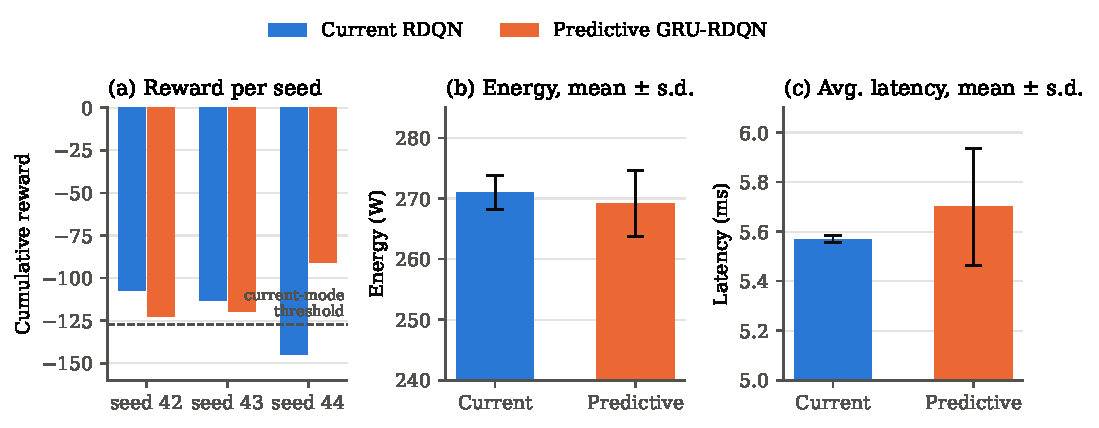
\includegraphics[width=\textwidth]{real_three_seed}
  \caption{E3 final test. (a) Reward of each seed; the dashed line is the current-mode threshold. (b, c) Mean $\pm$ sample s.d. of energy and average latency (axes truncated to show the differences).}
  \label{fig:real}
\end{figure}

Averaged over seeds, predictive GRU-RDQN achieved a better reward ($+10.61$), slightly lower energy ($-1.8$\,W) and fewer overload and underload steps. Current RDQN kept slightly lower average latency ($-0.13$\,ms) and a lower load index, and worst-case latency was identical. The per-seed results, however, show that the predictive advantage in mean reward comes from \emph{one} seed. Current RDQN was better for seeds 42 and 43, by 15.3 and 6.6 points, and predictive GRU-RDQN was better for seed 44, by 53.8 points. The between-seed standard deviations (about 18--20 points) exceed the mean difference. With three seeds, the honest conclusion is that the two modes are \emph{not distinguishable} on this trace. On average, each learned policy beat its same-mode threshold baseline: by 5.5 points in current mode and 22.6 in predictive mode. They did not do so on every seed, since current RDQN lost to threshold for seed 44 and predictive GRU-RDQN lost narrowly for seed 43.

Validation for E3 (Appendix~\ref{app:tables}) took place in an almost overload-free period ($\le0.2$\% of steps) in which all active policies were within about 2.5 reward points of each other. That validation period could not separate the models, and this probably contributes to the seed-to-seed variability of the selected checkpoints.

\section{Comparison with Existing Methods}
\label{sec:compare-existing}

The baselines in this study are threshold, random-valid and no-op policies implemented in the same environment; published algorithms were not re-implemented. A direct numerical comparison with published results is not valid, for three reasons:
\begin{enumerate}[leftmargin=*]
  \item The \emph{decision problems} differ. MOOO-RDQN~\cite{chen2025mooo}, DDCP~\cite{bouzidi2022ddcp} and AP-DQN~\cite{farahi2026apdqn} choose placements; SAR-LB~\cite{yeo2021sarlb} migrates among a fixed set of controllers; Li \emph{et al.}~\cite{li2024mec} place controllers and select edges in MEC.
  \item The \emph{traffic, controller counts and capacities} differ.
  \item The \emph{metrics} differ: those papers report percentage improvements over their own baselines, whereas this work reports a bounded reward together with absolute latency and modelled energy.
\end{enumerate}
For the same reason, latency and load values transcribed from the MOOO-RDQN paper into an early evaluation script were deliberately excluded from this report. They could not be verified and they measure a placement outcome, not a runtime policy.

The comparison that can be made is methodological (Table~\ref{tab:litcompare}). Relative to that literature, the distinctive elements of this work are listed below.
\begin{itemize}[leftmargin=*]
  \item \textbf{Joint runtime actions.} One policy chooses migrate, park, evoke or wait. The E1 results show the value of this combination: most of the learned policy's advantage over threshold control comes from \emph{energy}, which a migration-only policy such as SAR-LB cannot change, while overload is still handled through migration.
  \item \textbf{A matched forecast ablation.} Unlike forecast-assisted placement~\cite{li2024mec}, the same agent is trained with and without forecasts, which shows that the forecast's value depends on the topology and the traffic.
  \item \textbf{Evaluation discipline.} The study uses chronological splits, a single-use test set, baselines run under identical conditions, a zero-shot transfer test and multi-seed replication, as recommended for credible DRL evaluation~\cite{henderson2018matters,agarwal2021precipice}.
\end{itemize}
Conversely, those works include elements not covered here: controller placement itself, a real controller platform (ONOS in DDCP), formal safety layers~\cite{dinh2025safe} and multi-domain federated training~\cite{jha2026federated}.

\section{Ablation Studies and Additional Analyses}
\label{sec:ablation}

\subsection{Current-state versus predictive observation}
\label{sec:ablation-mode}

The main ablation removes the forecast input while keeping everything else identical: environment, reward, network, seed and budget. Table~\ref{tab:ablation-mode} shows the synthetic validation results that determined the observation mode for each topology.

\begin{table}[htbp]
\centering
\caption{Ablation on synthetic validation data: current RDQN versus predictive GRU-RDQN (horizons 5 and 3). Rewards in predictive mode are compared with the best predictive-mode baseline.}
\label{tab:ablation-mode}
\small
\fitwidth{\begin{tabular}{@{}llrrrrr@{}}
\toprule
\textbf{Topology} & \textbf{Model} & \textbf{Reward} & \textbf{Avg lat.} & \textbf{Energy} & \textbf{Load idx} & \textbf{F.-only acts}\\
\midrule
\multirow{3}{*}{Gridnet} & Current RDQN & \textbf{$-$440.90} & 8.81 & \textbf{411.31} & \textbf{0.807} & --\\
 & Predictive, $h=5$ & $-$493.40 & \textbf{8.02} & 418.78 & 1.072 & 2.67\\
 & Predictive, $h=3$ & $-$491.91 & 8.70 & 413.50 & 0.986 & --\\
\midrule
\multirow{3}{*}{BellCanada} & Current RDQN & \textbf{$-$399.99} & 11.74 & \textbf{405.85} & 8.405 & --\\
 & Predictive, $h=5$ & $-$441.32 & \textbf{11.25} & 439.45 & \textbf{7.316} & 2.50\\
 & Predictive, $h=3$ & $-$437.84 & 11.79 & 441.49 & 7.940 & --\\
\midrule
\multirow{2}{*}{OS3E} & Current RDQN & $-$480.22 & 5.12 & 441.19 & 3.729 & --\\
 & Predictive, $h=5$ & \textbf{$-$445.81} & \textbf{4.39} & \textbf{383.83} & \textbf{3.653} & 5.67\\
\bottomrule
\end{tabular}}
\par\smallskip\footnotesize ``F.-only acts'': successful actions per episode taken on forecast-only overload. Best predictive baselines on validation: Gridnet $-$513.55, BellCanada $-$462.27 ($h=5$) / $-$438.92 ($h=3$), OS3E $-$493.56.
\end{table}

On OS3E, prediction improved \emph{every} metric on validation. The predictive agent also used forecast-only actions most often there (5.67 per episode), and the improvement carried over to the final test, where predictive GRU-RDQN scored $-452.94$ against $-478.46$ for current RDQN and used 380.89\,W against 442.18\,W. Notably, current RDQN on OS3E had \emph{not} beaten the threshold policy ($-478.46$ versus $-474.79$ on test), so OS3E is the topology where forecasting made the difference between a learned policy that beats threshold control and one that does not. On Gridnet and BellCanada, prediction improved latency but lowered reward and raised energy compared with current RDQN, although it still beat every predictive-mode baseline. Mode comparisons across tables should be read with care, because predictive mode changes the valid-action sets and therefore the baselines' trajectories. The within-mode comparison is the strictly fair one.

\subsection{Forecast horizon}

Reducing the horizon from 5 to 3 (Table~\ref{tab:ablation-mode}) slightly improved predictive reward on Gridnet ($-493.40\rightarrow-491.91$) and BellCanada ($-441.32\rightarrow-437.84$), consistent with the more accurate horizon-3 forecasts (Table~\ref{tab:gru}). It did not close the gap to current RDQN, so horizon 5 was kept for OS3E and current mode was selected for Gridnet and BellCanada.

\subsection{Training budget on the largest topology}

With 80k steps, Cogentco current RDQN \emph{lost} on validation to no-op ($-538.46$ versus $-481.67$) and to threshold ($-524.98$), and used 452\,W. Retrained with 120k steps, it won on the final test ($-447.52$ against $-472.06$ for no-op) and used 374\,W, with fewer evokes (1.5 versus 2.7 per episode). The two numbers come from different splits, so they are not a controlled comparison. They are, however, consistent with the expectation that a 208-action problem needs more experience. Cogentco's training time (314\,min for 120k steps on CPU) also shows the cost of scaling a flat action space.

\subsection{Action behaviour and validity}

Across all reported final tests, both learned and baseline policies had \textbf{zero failed actions}, which confirms that the valid-action mask and feasibility checks work as intended. On synthetic traffic the learned policies performed 1.7--2.8 parks, 1.5--3.2 evokes and 24--57 migrations per 500-step episode, and took no action in the remaining 87--95\% of steps (Appendix~\ref{app:tables}). Compared with threshold control, they evoked less often on the large topologies; on Interoute, 1.7 versus 2.8 evokes per episode with fewer migrations, which explains most of the energy difference. The policies therefore learned \emph{when not to add capacity}, a judgement a fixed rule cannot make.

\subsection{Implementation verification}

Before any final experiment, an audit of an earlier version of the code found twelve defects, summarised in Appendix~\ref{app:verification}. They included traffic advancing only every 50 steps, evaluation always starting at the low-load start of the trace, rewards of about $\pm200$ outside the C51 support, probability mass lost in the C51 projection, unflushed $n$-step returns and state-dependent action indices. All results in this chapter were produced after these fixes with new models; pre-fix results are not reported. Eight regression tests now guard these invariants.

\section{Discussion of Findings}
\label{sec:discussion}

\paragraph{Objective O1 (environment).} The environment reproduces the intended decision problem across five real topologies of very different size. Its valid-action mechanism eliminated failed actions for all policies, and its stable action schema and versioned checkpoints made results reproducible and kept incompatible models from being evaluated.

\paragraph{Objective O2 (learning and fair evaluation).} On held-out synthetic traffic, Rainbow DQN learned controller-management policies that beat threshold, random-valid and no-op control in reward on all five topologies. The main mechanism is energy-aware restraint: keeping fewer controllers active, adding capacity only when it pays off, and still resolving overload by migration. The cost is a small increase in average latency on most topologies. This is the trade-off the reward was designed to make, not a defect, but a deployment that prioritises latency would need different weights.

\paragraph{Objective O3 (forecasting).} Forecasting helped where the forecaster was accurate \emph{and} the policy used it. OS3E had the most forecast-only actions and the largest gain. It did not help on Gridnet and BellCanada despite good forecasts, which suggests that the extra 15--54 state dimensions made learning harder within the same 80k-step budget. On real traffic the evidence was neutral: averaged over three seeds predictive mode was ahead, but one seed drove that difference. The answer to O3 is therefore conditional: \emph{a GRU forecast can make controller management more proactive and more energy-efficient, but its benefit depends on the topology, the forecast quality and the traffic regime, and it is not universal.}

\paragraph{Limitations and threats to validity.}
\begin{itemize}[leftmargin=*]
  \item \emph{Construct validity.} Latency is graph propagation delay only; queueing and controller processing delay are not modelled. Energy is a three-level state model. Controller capacity is represented by fixed normalised thresholds.
  \item \emph{External validity.} The synthetic generator, although stress-oriented and topology-scaled, is not operator traffic. The real-traffic study maps 12 Abilene nodes onto 34 OS3E switches through a fixed projection and covers one topology. No OpenFlow controller or Mininet deployment was used.
  \item \emph{Statistical validity.} The synthetic results use one training seed, and E3 uses three. Within-evaluation reward variance is large, and per-window results were not stored for paired testing. No significance claims are made.
  \item \emph{Internal validity.} Selection decisions used validation data only, and test splits were used once. The Cogentco 120k model lacks a recorded validation run, and E3 validation was too quiet to discriminate between models. The reward weights and thresholds were fixed by design and not tuned, and their sensitivity is untested.
  \item \emph{Scalability.} A separate agent is trained per topology, and the flat action space grows with $N$, which makes training on large networks expensive on CPU.
\end{itemize}
These limitations bound the claims made in this report. They do not undermine the central result, which rests on matched comparisons inside a single, documented environment.
